%!TEX root = ../report.tex

\section{Technical non-functional requirements}
This section describes the technical aspects that are important to the system as requirements. These requirements determine various APIs and programs that the system will rely on.

% In this section, the technical non-functional requirements important to this system are discussed.

\subsection{Reliability}
% The response time should be about NUMBER mS
% Failure rate ?
% Data transmission
% The margin of error tolerated has to be as low as possible .\\ GK: Margin of error in what aspect?
Reliability is an important non-functional requirement for the system, and a key-driver of the architecture as well.
\begin{longtable}{L{0.1\textwidth} L{0.12\textwidth} L{0.7\textwidth}}
	\textbf{Nr.} & \textbf{Prio}  & \textbf{Description} \\
	%\reqRow{rel}{Must}{Sensor sites are equipped with at least two sensors} ( why two ? )
	\reqRow{rel}{Must}{Data from the sensors reaches the central server in 99.9\% of all cases} % Already mention REST here?
	 
	\reqRow{rel}{Must}{The system must detect if a sensor supplies wrong measurements, which can be caused, e.g. by improper calibration or defects in the sensor.} 
	
	\reqRow{rel}{Must}{The system must at no time fail to detect a flood when this flood becomes imminent (\textit{false negative}).}
	
	\reqRow{rel}{Must}{The system must not detect a flood, when this flood is not there in reality (\textit{false positive}), on average more than once per 5 years.}
	 
	%\reqRow{rel}{Must}{Redundancy} % GK: if redundancy is required, which it should be, in what way?
	%This means adding redundancy to the system so that failure of a component does not mean failure of the entire system
	\bottomrule
\end{longtable}

\subsection{Availability}
\begin{longtable}{L{0.1\textwidth} L{0.12\textwidth} L{0.7\textwidth}}
	\textbf{Nr.} & \textbf{Prio}  & \textbf{Description} \\
	\reqRow{ava}{Must}{The system must have an uptime of $99.7\%$. This effectively means, that the system should not be down for more than 2 hours per month. $AV = \frac{\text{MTTF}}{\text{MTTF} + \text{MTTR}} = \frac{\text{6 months}}{\text{6 months }+\text{ 12 hours}} = \frac{4380 \text{ hours}}{4380 + 12 \text{ hours}} = 99.7 \%$}

	\reqRow{ava}{Must}{The system must not experience a period of downtime, spanning more than 12 hours. Within twelve hours of the system going offline, it should be back up again. }
	\reqRow{ava}{Must}{The system pulls weather forecasts from at least two weather forecasting services.}
	\bottomrule
\end{longtable}


\subsection{Resilience}
The system needs to be resilient to recover from errors and mistakes without impacting the systems functionality.
\begin{longtable}{L{0.1\textwidth} L{0.12\textwidth} L{0.7\textwidth}}
	\textbf{Nr.} & \textbf{Prio}  & \textbf{Description} \\
	
	\reqRow{res}{Must}{The system recognizes failures within half an hour}

	\reqRow{res}{Must}{The system recovers from failures without the \qos or the functionality of the system being affected.}
	
	\reqRow{res}{Must}{All system data must be backed up every 24 hours.}
	
	\reqRow{res}{Must}{In case of a data loss, the data should be retrieved and restored from a backup within 2 hours.}
	
	\reqRow{res}{Must}{Backup copies are stored in a secure location which is not in the same area as the system (50 km away).}
	
	\bottomrule
\end{longtable}

\subsection{Performance}

\begin{longtable}{L{0.1\textwidth} L{0.12\textwidth} L{0.7\textwidth}}
	\textbf{Nr.} & \textbf{Prio}  & \textbf{Description} \\
	\reqRow{perf}{Must}{Data is transmitted from and to the system with a minimum average speed of 10 megabits per second} % How to calculate GK: Doesn't really matter for requirements, but good to think about. Also: response time to what? Request? Detecting floods? Furthermore, 10 (just saying something) GB of data is not transferable witihin 1 second if you include connection setup time etc etc
	% GK: only about datatransmission express in dataspeed
	
	\reqRow{perf}{Must}{The data transmission between the sensors and the system is on average at least 10 megabits per second for each sensor.}
	% How many data the system can receive in one second ?
	\reqRow{perf}{Must}{The time for the system to compute if there is a flood or not according to a critical level and the data received from the sensors is at most 5 minutes. }
	
	\reqRow{perf}{Must}{ If an imminent flood is detected, the warning text message to citizens arrives in 5 minutes. }
	
	\reqRow{perf}{Must}{ If an imminent flood is detected, the warning to the safety region arrives within 1 minute. }

	\bottomrule
\end{longtable}
% GK: requirement for amount of concurrent users

%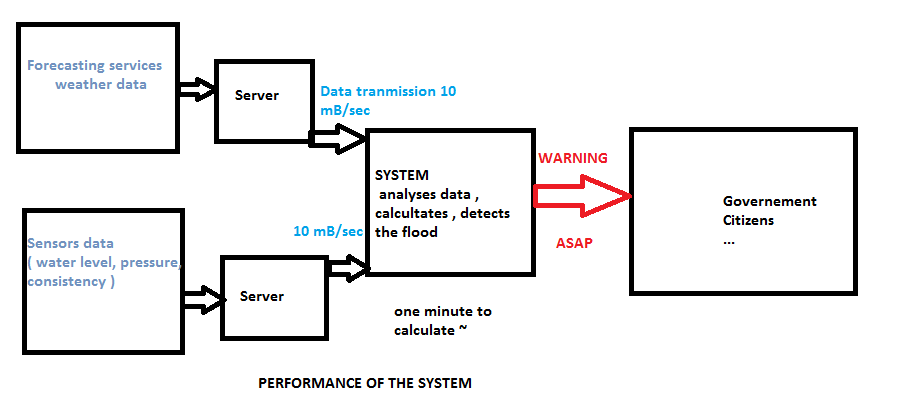
\includegraphics[scale=0.7]{3-requirements/Images/Performance.jpg}

\subsection{Interoperability}
The system has dependencies on several third-party systems and also allows third parties to retrieve information from it.

\begin{longtable}{L{0.1\textwidth} L{0.12\textwidth} L{0.7\textwidth}}
	\textbf{Nr.} & \textbf{Prio}  & \textbf{Description} \\
	
	%\reqRow{intr}{Must}{When the system detects a high risk of flood, it warns the government automatically using the government provided API.} WM: removed this, the safety region will warn the government (mayor etc.)
	%\reqRow{intr}{Must}{When the system detects a flood, it notifies the safety region through an API provided by them.}
	%\reqRow{intr}{Must}{The system sends out a SMS to all users who are subscribed to flood warnings using the mobile network.}
	\reqRow{intr}{Must}{The system is able to retrieve data from different types of sensors.}
	\reqRow{intr}{Must}{The system is able to retrieve external data from different APIs.}
	%\reqRow{intr}{Must}{The system exposes an API, allowing third parties to develop applications using the systems data.}
	% \reqRow{intr}{Must}{The sensors are able to communicate with the system using a mobile broadband connection.} REMOVED: because we have decided to use wired connection later on.

	\bottomrule
\end{longtable}
\todo[inline]{intr-6 Not measurable}
% GK; Requirement about working with different kind of sensors for the same data

\subsection{Security}
The security of the system is very relevant to its success. The system should be secure, because unauthorized access can have a big impact on society (when e.g. false flood warnings are triggered).
\begin{longtable}{L{0.1\textwidth} L{0.12\textwidth} L{0.7\textwidth}}
	\textbf{Nr.} & \textbf{Prio}  & \textbf{Description} \\
	\reqRow{sec}{Must}{Access to the system is restricted to users, which are authorized and authenticated using a password protected user account.}
	\reqRow{sec}{Must}{All communication to, from and within the system is encrypted.}
	\reqRow{sec}{Must}{User account information is stored encrypted.} %hashed using bcrypt after being salted with 128 randomly generated characters.
	\reqRow{sec}{Must}{The system is protected on both the application layer and network layer.}
	% WM: does communication within the system mean between the different components of the system?
	\reqRow{sec}{Must}{The system communicates with the sensors via a secure HTTPS connection.} % Do we want to communicate with the sensors via REST? WM: Could this be more generic? Like: 'the system communicates with the sensors via a secure connection'

	\bottomrule
\end{longtable}
% TODO: how to measure?

\subsection{Scalability}
The system has to be designed in a way that it can expand over time. Not only should it span larger geographic areas, but more functionality will be added later as well.
% The system will be able to cover more areas and use more sensors in the future. GK: too vague, but added scale-3 based on this idea
\begin{longtable}{L{0.1\textwidth} L{0.12\textwidth} L{0.7\textwidth}}
	\textbf{Nr.} & \textbf{Prio}  & \textbf{Description} \\
	\reqRow{scale}{Must}{The database and services of the system can scale within 1 hour, when the systems resource usage increases.}

	\reqRow{scale}{Must}{The system is configurable to run in different areas and with different sensors.}
	
	\reqRow{scale}{Must}{The system maintains the performance requirements when the geographic area the system covers is expanded.}
	
	\bottomrule
\end{longtable}
% The system will be developed with more sensors and in more places.
%New functionalities, for example GPS
% ============================================================
% From Gerrit:
% The three main requirements:
% 1: Monitoring activities: the system should monitor activities and properties of
% rivers, waterways, dykes, such as the water level and pressure or the consistency
% of the dyke. Monitoring can be performed through different devices, e.g. analog
% and digital sensors, Unmanned Aerial Vehicles (UAVs) and Vehicular Ad-hoc
% Networks (VANETs) etc.
% 2: Warning: in case of an imminent flood, the system should issue warnings to the
% authorities and emergency services, but also directly to citizens who are
% subscribed for such messages (e.g. through SMS or mobile apps).
% 3: Guidance: the system should provide runtime information to guide its
% constituents or third parties, .e.g. the UAVs may provide information to
% VANETs embedded in vehicles crossing the area, thereby guiding vehicles
% driving towards a flood area to avoid certain routes. Meanwhile, the VANETs
% can also provide an alternative route to emergency services or citizens to avoid
% the flood area. 
% ToDo:
% Stakeholders
% Use-cases
% Make them smart
% Assign value (must/should/...
% ============================================================